\section{Техническое задание}
\subsection{Основание для разработки}

Полное наименование системы: «Программно-информационная система для оценки и контроля знаний».
Основанием для разработки программы является приказ ректора ЮЗГУ
от «17» апреля 2025 г. №1828-с «О направлении (допуске) на практику».

\subsection{Цель и назначение разработки}

Программно-информационная система предназначена для контроля и оценки знаний обучающихся с целью улучшения процесса обучения.

Задачами данной разработки являются:
\begin{enumerate}
\item создание модуля для создания новых тестов;
\item создание модуля для создания вопросов;
\item создание модуля для редактирования вопросов;
\item создание модуля для авторизации;
\item создание модуля для регистрации;
\item создание модуля для просмотра результатов пройденных тестов;
\item создание модуля для управления пользователями;
\item создание модуля для пользователя;
\item создание модуля для администратора;
\item реализация системы оценивания по результатам теста;
\item реализация системы хранения тестов и результатов тестов;
\end{enumerate}

\subsection{Требования к данным программной системы}

Входными данными для системы являются:
\begin{itemize}
    \item данные имеющихся тестов;
    \item данные о зарегистрированных пользователях;
    \item данные администратора;
\end{itemize}

Выходными данными для системы являются:
\begin{itemize}
	\item графическое отображение вопросов тестов;
	\item данные создании/изменении тестов;
	\item данные о новых зарегистрированных/добавленных администратором пользователях;
	\item данные о изменении паролей пользователей;
	\item данные результатов пройденных тестов.
\end{itemize}

\subsection{Функциональные требования к программной системе}

В разрабатываемой программно-информационной системе должно
быть предусмотрено наличие два класса пользователей: пользователь и администратор.

Пользователю должны быть доступны следующие функции программы:
\begin{enumerate}
	\item Авторизация.
	\item Регистрация.
	\item Прохождение выбранного теста.
	\item Просмотр собственных результатов пройденных тестов.
\end{enumerate}

Администратору должны быть доступны следующие функции программы:
\begin{enumerate}
	\item Авторизация.
	\item Изменение пароля администратора.
	\item Прохождение выбранного теста.
	\item Просмотр результатов всех пользователей.
	\item Управление пользователями.
	\item Создание новых тестов.
	\item Редактирование имеющихся тестов.
\end{enumerate}

\subsection{Моделирование вариантов использования}

Для разрабатываемой системы тестирования знаний была реализована модель, которая обеспечивает наглядное представление вариантов использования системы.

Она помогает в физической разработке и детальном анализе взаимосвязей объектов.

Диаграмма вариантов описывает функциональное назначение разрабатываемой системы. То есть это то, что система будет непосредственно делать в процессе своего функционирования. Она является исходным концептуальным представлением системы в процессе ее проектирования и разработки. Проектируемая система представляется в виде ряда прецедентов, предоставляемых системой актерам или сущностям, которые взаимодействуют с системой. Актером или действующим лицом является сущность, взаимодействующая с системой извне (например, человек, техническое устройство). Прецедент служит для описания набора действий, которые система предоставляет актеру.

\clearpage

На рисунке ~\ref{user_precedent_diagram:image} в виде диаграммы прецедентов представлены функциональные требования к системе, доступные для пользователя.

\begin{figure}[H]
	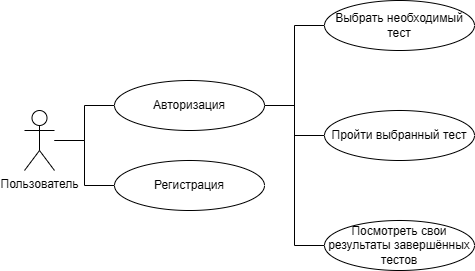
\includegraphics[width=1\linewidth]{диаграмма_прецедентов_пользователь}
	\caption{Диаграмма прецедентов пользователя}
	\label{user_precedent_diagram:image}
\end{figure}

\clearpage

На рисунке ~\ref{admin_precedent_diagram:image} представлены дополнительные функциональные требования к системе для администратора.

\begin{figure}[H]
	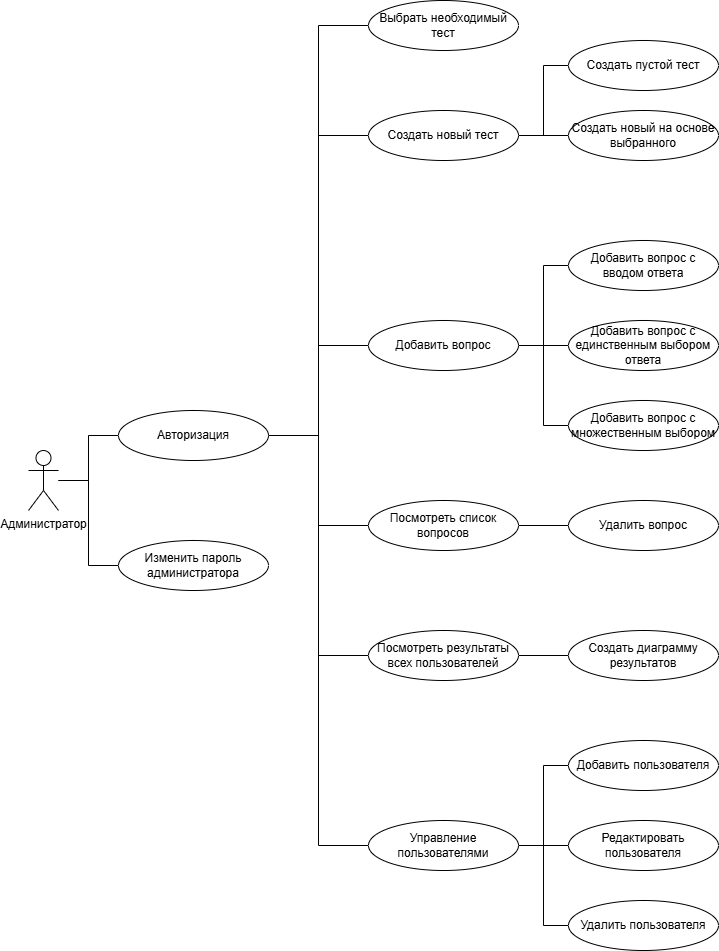
\includegraphics[width=1\linewidth]{диаграмма_прецедентов_администратор}
	\caption{Диаграмма прецедентов администратора}
	\label{admin_precedent_diagram:image}
\end{figure}

На основании анализа предметной области в программе должны быть реализованы следующие варианты использования: 
Для пользователя:
\begin{enumerate}
\item ВИ "Авторизация". Данный прецедент позволяет пользователю авторизоваться.
\item ВИ "Регистрация". Данный прецедент позволяет зарегистрироваться.
\item ВИ "Выбрать желаемый тест". Данный прецедент позволяет пользователю выбрать желаемый тест.
\item ВИ "Пройти выбранный тест". Данный прецедент позволяет пользователю приступить к прохождению выбранного теста.
\item ВИ "Добавить вопрос". Данный прецедент позволяет пользователю добавить вопрос в выбранном тесте.
\item ВИ "Удалить вопрос". Данный прецедент позволяет пользователю удалить вопрос в выбранном тесте.
\item ВИ "Просмотреть результаты". Данный прецедент позволяет пользователю посмотреть собственные результаты пройденных тестов.
\item ВИ "Создать новый тест". Данный прецедент позволяет пользователю создать новый тест.
\end{enumerate}

Для администратора:
\begin{enumerate}
	\item ВИ "Авторизоваться как администратор". Данный прецедент позволяет авторизоваться как администратор и получить соответствующие права.
	\item ВИ "Изменить пароль администратор". Данный прецедент позволяет изменить пароль администратор. Требуется ввести старый пароль и два раза повторить новый.
	\item ВИ "Выбрать желаемый тест". Данный прецедент позволяет администратору выбрать желаемый тест.
	\item ВИ "Пройти выбранный тест". Данный прецедент позволяет администратору приступить к прохождению выбранного теста.
	\item ВИ "Добавить вопрос". Данный прецедент позволяет администратору добавить вопрос в выбранном тесте. Возможно добавить три варианта вопроса: с вводом ответа, с единственным выбором из имеющихся ответов, с множественным выбором из имеющихся ответов.
	\item ВИ "Просмотреть набор выбранного теста". Данный прецедент позволяет администратору посмотреть состав теста.
	\item ВИ "Удалить вопрос". Данный прецедент позволяет администратору удалить выбранный вопрос.
	\item ВИ "Просмотреть результаты". Данный прецедент позволяет администратору посмотреть результаты пройденных тестов всех пользователей.
	\item ВИ "Создать новый тест". Данный прецедент позволяет администратору создать новый тест. Можно создать пустой тест или копировать текущий набор выбранного теста.
	\item ВИ "Управление пользователями". Данный прецедент позволяет администратору добавить нового пользователя, удалить или редактировать уже существующего.
\end{enumerate}

\subsection{Описание вариантов использования}

Данные варианта использования "Пройти выбранный тест".

Входными данными является выбранный тест, имя пользователя.

Выходными данными прецедента "Пройти выбранный тест" являются вопросы с ответами и результат прохождения теста.

Основной исполнитель: Пользователь.

Заинтересованные лица и их требования: Пользователь хочет пройти тест.

Предусловие: поля для ввода имени, ответа на вопрос должны быть заполнены.

Постусловие: приложение проверит введены ли данные, если нет, сообщит об этом пользователю.

Основной успешный сценарий:
\begin{enumerate}
	\item Пользователь запускает программу.
	\item Пользователь проходит авторизацию, введя своё имя.
	\item Пользователь попадает в меню.
	\item Пользователь выбирает желаемый тест.
	\item Пользователь нажимает кнопку "Пройти тест".
	\item Пользователь попадает в окно теста.
	\item Пользователь выбирает или вводит ответы.
	\item Пользователь по окончании теста видит его результат.
	\item Пользователь закрывает приложение.
\end{enumerate}

Данные варианта использования "Создать новый тест".

Входными данными является пароль администратора, данные для нового теста.

Выходными данными прецедента "Создать новый тест" являются новый тест с вопросами и ответами.

Основной исполнитель: Администратор.

Заинтересованные лица и их требования: Администратор хочет создать тест и добавить в него вопрос

Предусловие: поля для ввода пароля администратора, текста вопроса и его ответа должны быть заполнены.

Постусловие: приложение проверит введены ли данные, если нет, сообщит об этом администратору.

Основной успешный сценарий:
\begin{enumerate}
	\item Администратор запускает программу.
	\item Администратор проходит авторизацию, введя пароль.
	\item Администратор попадает в меню.
	\item Администратор нажимает кнопку "Создать тест".
	\item Администратор попадает в окно создания теста".
	\item Администратор нажимает кнопку "Создать новый тест".
	\item Администратор нажимает кнопку "Вернуться в меню".
	\item Администратор попадает в меню.
	\item Администратор нажимает кнопку "Добавить вопрос".
	\item Администратор попадает в меню добавления вопроса.
	\item Администратор нажимает кнопку добавить базовый вопрос.
	\item Администратор в окне создания базового вопроса вводит текст и ответ вопроса.
	\item Администратор нажимает кнопку добавить вопрос.
	\item Администратор закрывает приложение.
\end{enumerate}

\subsection{Требования к оформлению документации}

Разработка программной документации и программного изделия должна производиться согласно ГОСТ 19.102-77 и ГОСТ 34.601-90. Единая система программной документации.
